\capitulo{3}{Conceptos teóricos}


Se detallan a continuación los conceptos relevantes que se han considerado necesarios a incluir en esta sección.

\section{Glucosa e insulina}

\subsection{La glucosa}

La glucosa es un carbohidrato con fórmula empírica $ C_6H_{12}O_6$ que pertenece al grupo de las aldohexosas, pues contiene 6 átomos de carbono y presenta una aldosa.  Su grupo carbonilo se encuentra en el carbono 1 de la cadena carbonada.
Puede encontrarse de forma libre o combinada, y es el compuesto orgánico más abundante en la naturaleza. Su importancia radica en ser la principal fuente de energía de las células, realizando funciones como la oxidación catabólica. Además, es el componente principal de polímeros de gran importancia estructural como la celulosa, así como de polímeros de almacenamiento energético como el almidón o el glucógeno.


A nivel estructural, presenta más de una configuración, visible en la Figura \ref{fig:formula_glucosa} y obtenida de \cite{murray2007bioquimica}. Su forma lineal se compone de una cadena recta (aldohexosa), tal y como se ha definido al comienzo de la sección por su fórmula empírica. Además, puede encontrarse de forma cíclica, mediante un hemiacetal formado por reacción entre el grupo aldehído y el grupo hidroxilo. Esta configuración es favorecida en el aspecto termodinámico, y se dibuja mediante la proyección de Haworth resultando una estructura en anillo, de seis miembros, con los grupos hidroxilo situados por arriba o por debajo del plano.

\begin{figure}[h]
    \centering
    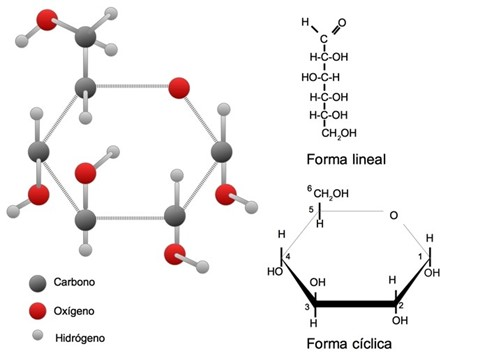
\includegraphics[width=0.7\textwidth]{img/imagen_formula_glucosa.jpg}
    \caption{Configuraciones de la glucosa.}
    \label{fig:formula_glucosa}
    \vspace{0.5cm} % Ajusta el espacio vertical entre la imagen y el texto
\end{figure}

La glucosa es el carbohidrato más simple, lo que lo convierte en un monosacárido e implica la presencia de azúcar. Sin embargo, otros monosacáridos también contienen azúcar, como la ribosa, la galactosa o la fructosa, con la que comparte fórmula, y respecto a la que se diferencia por la posición relativa de sus grupos -OH y O=.  
Presenta dos formas, la D- Glucosa y la L- Glucosa. La D-(+)-glucosa es uno de los compuestos más importantes para los seres vivos, incluyendo a seres humanos.
La glucosa en sangre es el principal azúcar de la sangre, y es la principal fuente de energía del cuerpo humano. Se obtiene de la ingesta de alimentos, y cuando estos se procesan, el azúcar pasa al torrente sanguíneo, por donde circula libre, y se almacena en forma de glucógeno. Entre sus funciones, destacan dos:

\begin{enumerate}
    \item[-] Obtención de energía, mediante su transformación a adenosín trifosfato (ATP) dentro de las células.
    \item[-] Reserva de energía, si el cuerpo no necesita su energía de forma inmediata, se almacena en forma de glucógeno en hígado y músculos.
\end{enumerate}

Los niveles de azúcar en sangre se encuentran dentro de unos rangos que garantizan el correcto funcionamiento del organismo. Los rangos infereriores suelen venir delimitados por la glucosa basal, que es el nivel de glucosa en ayunas, y cantidades muy inferiores a ella comprometen la estabilidad del organismo, causando hipoglucemia. El efecto contrario se denomina hiperglucemia. Estos niveles se regulan mediante una hormona denominada insulina. Además, esta hormona participa en el transporte de glucosa desde el torrente sanguíneo a las células, donde se utiliza la glucosa como energía.


\subsection{La insulina}

La insulina humana es una hormona de naturaleza proteína sintetizada en las células beta de los islotes de Langerhans del páncreas. Fue descubierta en 1921 y es secretada en respuesta a niveles elevados de glucosa, así como ante algunas hormonas peptídicas como el glucagón o la secretina.

Es una proteína globular muy conservada compuesta por 51 aminoácidos en su forma activa, como se muestra en la Figura \ref{fig:insulina_quimica} \footnote{Obtenido de \cite{insulina_website}}. En su centro proteico se encuentran los aminoácidos no polares, formando un núcleo hidrofóbico, mientras que los aminoácidos polares y cargados se sitúan alrededor del núcleo. Estos se distribuyen en 2 cadenas, A y B, de 21 y 30 aminoácidos respectivamente. Ambas cadenas interaccionan mediante puentes disulfuro.

\begin{figure}[h]
    \centering
    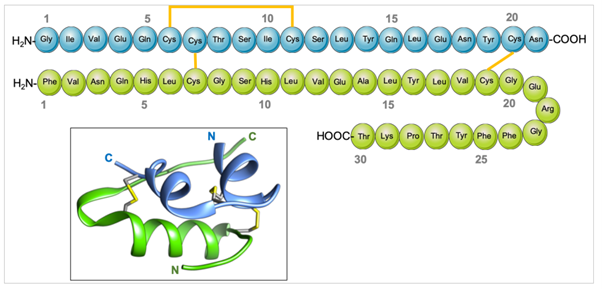
\includegraphics[width=0.7\textwidth]{img/imagen_insulina.png}
    \caption{Disposición de los aminoácidos de la insulina.}
    \label{fig:insulina_quimica}
\end{figure}

Las células del organismo, sin embargo, tienen dificultades para hacer que las proteínas se plieguen de forma correcta en estructuras estables. Como solución, se sintetiza una proteína más grande llamada proinsulina, en la Figura \ref{fig:proinsulina}.

El ARN mensajero de la insulina se traduce como un precursor de una cadena polipeptídica llamada preproinsulina, compuesta por 110 aminoácidos. Esta cadena, tras eliminarse su péptido señal durante su inserción en el retículo endoplasmático, da lugar a la proinsulina. Cuenta con 87 residuos y se modifica en el Aparato de Golgi. De él salen las vesículas secretoras con la hormona activa, la insulina.
A nivel estructural, la proinsulina presenta 3 dominios: una cadena de la amino terminal de la cadena B, con una alfa hélice;una cadena carboxi- terminal A con dos alfas hélices, y un péptido que conecta ambas conocido como péptido C.


\begin{figure}[h]
    \centering
    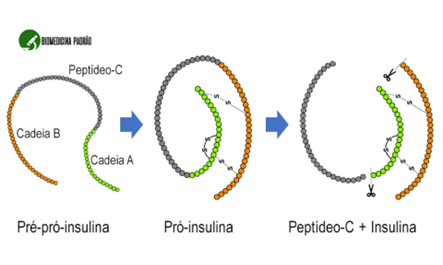
\includegraphics[width=0.7\textwidth]{img/imagen_proinsulina.png}
    \caption{Síntesis de insulina mediante proinsulina y el péptido C.}
    \label{fig:proinsulina}
\end{figure}

Por tanto, la insulina se sintetiza como preproinsulina. Esta molécula está formada por una sola cadena polipeptídica, que posteriormente y en diversas partes de la célula, sufre varios procesamientos para obtener finalmente la insulina activa.

Entre las funciones de la insulina, destacan dos. Por una parte, disminuye el nivel de glucosa sanguínea, como se ha comentado, favoreciendo la conversion de glucosa en glucógeno en los hepatocitos y miocitos siempre y cuando la glucosa se encuentre elevada. Por la otra parte, estimula la captación de glucosa en varios tipos de células, así como el almacenamiento y consumo de ésta en numerosos tejidos del cuerpo, y especialmente en músculos, tejido adiposo e hígado. Mientras que en el músculo incrementa el transporte de glucosa hacia el interior de las células musculares (que se consumirá para obtener energía en forma de ATP), en el hígado la insulina facilita la entrada de glucosa en células hepáticas, evita la liberación de glucosa a la sangre y promueve la síntesis de glucógeno. Así, en el tejido adiposo la insulina promueve, de forma indirecta, el depósito de grasas en forma de triglicéridos.
La acumulación de glucógeno en el hígado y de grasas en el tejido adiposo permite que el cuerpo tenga reservas de energía que poco a poco consumen durante el tiempo de ayunas para mantener una glucemia constante. Una vez que el organismo vuelve a estos valores normales de glucosa, se elimina la señal que provocó la síntesis de insulina, y esta deja de secretarse. La insulina también tiene, al igual que la glucosa, un valor basal, que delimita el rango inferior del comportamiento óptimo del organismo. Por debajo de este valor, se generan grandes riesgos para el metabolismo y funcionamiento celular adecuado.

\subsubsection{Insulina activa y concentración de insulina en sangre}

En este análisis se diferencian dos tipos de insulina:
\begin{enumerate}
    \item[-] \textit{Insulina}, se refiere a la cantidad total de insulina presente en el torrente sanguíneo en un momento dado. Puede medirse directamente mediante análisis de sangre, y representa tanto la insulina activa como cualquier otra forma de insulina presente en la sangre, ya sea unida a proteínas transportadoras, en forma de precursor inactivo o en cualquier otra forma.
    es la forma de la hormona que se secreta inicialmente por las células beta del páncreas en respuesta a un aumento en los niveles de glucosa en sangre. La insulina se secreta en su forma precursora, conocida como proinsulina, que luego se procesa para convertirse en insulina activa y péptido C gracias a una enzima específica llamada convertasa de prohormona (PC), que escinde el péptido C de la proinsulina.
    \item[-] \textit{Insulina activa}, se refiere específicamente a la fracción de insulina que está disponible para unirse a los receptores de insulina en los tejidos periféricos y ejercer su efecto biológico. Es la forma de insulina que ha sido procesada a partir de proinsulina, forma precursora de la insulina. 
\end{enumerate}


\section{Sistema glucorregulatorio}

Se denomina sistema glucorregulatorio al conjunto de mecanismos y procesos fisiológicos que el cuerpo utiliza para mantener los niveles de glucosa en la sangre dentro de un rango adecuado y saludable. Este sistema es crucial para el funcionamiento normal del organismo, ya que la glucosa es la fuente primaria de energía para las células; y se compone tanto de órganos como de hormonas.

\subsection{Actores principales en la glucorregulación}

El páncreas es el órgano principal en la regulación de la glucosa sanguínea. Contiene unas células especializadas llamadas células alfa y beta, situadas en los islotes de Langerhans (Figura \ref{fig:islotes} 
 \footnote{Obtenido de \cite{britannica_islets}}). Estas células secretan hormonas, la insulina y el glucagón, que están directamente implicadas en la variación de los niveles de glucosa en el organismo. 
\begin{figure}[h]
    \centering
    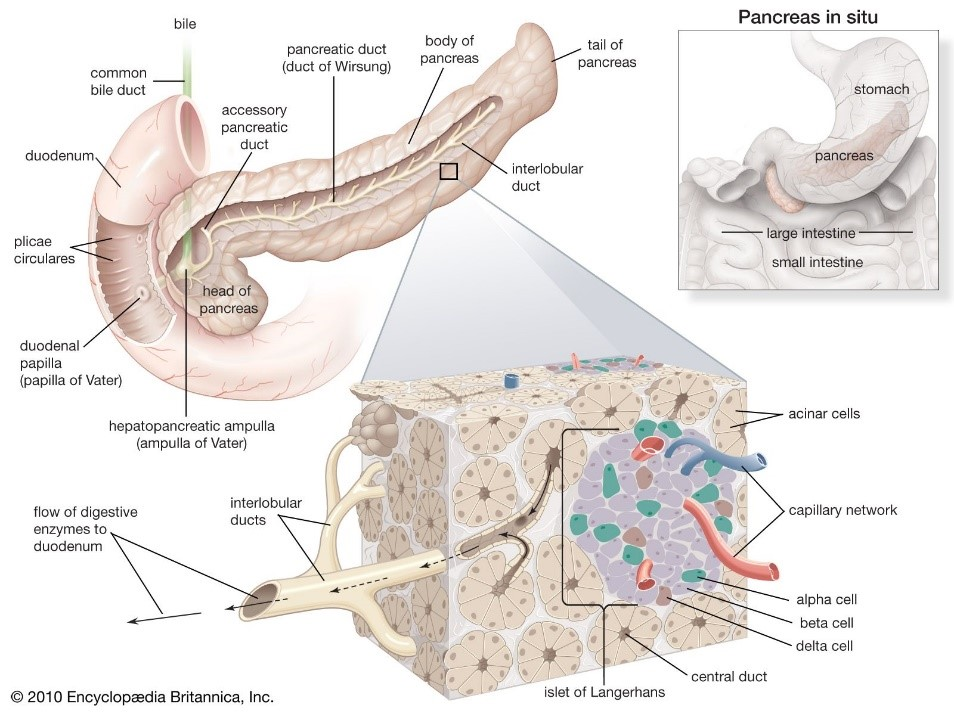
\includegraphics[width=0.8\textwidth]{img/imagen_islotes_langerhans.jpg}
    \caption{Islotes de Langerhans del páncreas y células beta y alfa.}
    \label{fig:islotes}
\end{figure}

Por su parte, el hígado almacena la glucosa en forma de glucógeno, y la libera cuando es necesario (ver Figura \ref{fig:basico_glucorregulatorio} \footnote{Obtenido de \cite{labster_glucose}}). También funcionan como depósito de almacenamiento de glucosa el músculo y tejido adiposo. El sistema nervioso central participa en la regulación de la glucosa mediante señales hormonales y nerviosas.
A nivel hormonal, son dos las hormonas principales del sistema glucorregulatorio. Por una parte, la insulina, como ya se ha comentado, es liberada por las células beta del páncreas cuando los niveles de glucosa en sangre son elevados. Facilita la entrada de glucosa a las células, especialmente en el hígado, músculos y tejido adiposo, para ser utilizada como energía o almacenada como glucógeno. Además, inhibe la producción de glucosa por el hígado (gluconeogénesis) , estimula la síntesis de glucógeno (glucogénesis) y facilita la conversión de glucosa en ácidos grasos para su almacenamiento.

La regulación del metabolismo de la glucosa por la insulina depende de un equilibrio muy delicado con otra hormona “hermana”, el glucagón, que se libera cuando los niveles de glucosa en sangre son bajos, generalmente durante la noche y entre las comidas, estimulando la conversión de glucógeno en glucosa en el hígado (gluconeogénesis), e inhibiendo la síntesis de glucógeno. 

Otras hormonas relevantes implicadas en el control de los niveles de glucosa en sangre son:
\begin{enumerate}
    \item[-] La adrenalina o epinefrina, producida por las glándulas suprarrenales, aumenta rápidamente los niveles de glucosa en respuesta al estrés. Actúa directamente sobre el hígado para promover la producción de azúcar, y promueve la descomposición y liberación de los nutrientes de la grasa que viajan hacia el hígado y que se convierten en azúcar y cetonas.
    \item[-] El cortisol es una hormona esteroide también secretada por la glándula suprarrenal que asimismo aumenta los niveles de glucosa en respuesta al estrés prolongado. En circunstancias normales, el cortisol compensa la acción de la insulina, pero bajo condiciones de estrés los niveles de cortisol se vuelven elevados y se adquiere insulino - resistencia. Bajo esta condición, las células del cuerpo no responden correctamente a la insulina, por lo que se necesita mayor cantidad de esta para lograr el mismo efecto de reducción de glucosa en sangre.
    \item[-] La hormona de crecimiento se libera desde la glándula pituitaria, en el cerebro, y compensa el efecto de la insulina sobre las células grasas y los músculos. Altos niveles de hormona de crecimiento provocan resistencia a la acción de la insulina.
    \item[-] Otras hormonas como las incretinas GLP-1 y GIP se producen en las células del intestino y potencian la secreción de insulina tras la ingesta, así como la amilina, cuyo efecto es muy similar.
\end{enumerate}
Pese a que esta hormonas quedan fuera del estudio presente, sería interesante comprender su funcionamiento en otros futuros análisis.

\subsection{Funcionamiento del sistema glucorregulatorio}
El sistema se rige por la variación de los niveles de glucosa en el organismo. 
Después de una comida, ver Figura \ref{fig:basico_glucorregulatorio} \footnote{Obtenido de \cite{velasquez2013modelado}.}, los niveles de glucosa se ven aumentados, lo que estimula a las células beta del páncreas a liberar insulina. Así, la glucosa de los alimentos se absorbe y llega a la sangre. La insulina la transporta a las células, donde se utiliza para ser almacenada en forma de glucógeno, ácidos grasos y aminoácidos. Como resultado, los niveles de glucosa en sangre disminuyen a niveles normales. Entre comidas, los niveles de glucosa en sangre comienzan a caer. Esta disminución estimula a las células alfa del páncreas a liberar glucagón. El glucagón actúa principalmente en el hígado, donde estimula la descomposición del glucógeno en glucosa, lo que aumenta los niveles de glucosa en sangre a niveles normales.

\begin{figure}[h]
    \centering
    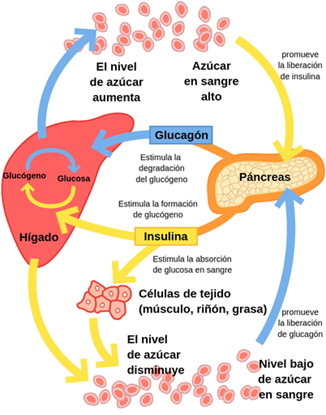
\includegraphics[width=0.5\textwidth]{img/imagen_funcionamiento_basico_glucosa.png}
    \caption{Funcionamiento básico de la regulación glucosa- insulina en el organismo.}
    \label{fig:basico_glucorregulatorio}
\end{figure}

Durante el ejercicio, la demanda de energía en los músculos aumenta, lo que provoca un mayor uso de glucosa. En respuesta, las glándulas suprarrenales liberan adrenalina, que estimula la liberación de glucosa y ácidos grasos para proporcionar energía rápida. Además, la adrenalina inhibe la liberación de insulina y estimula la liberación de glucagón, asegurando que haya suficiente glucosa disponible para satisfacer las necesidades energéticas del cuerpo.

\subsection{Alteraciones del sistema glucorregulatorio}

El equilibrio preciso y dinámico de los mecanismos que regulan la glucosa es esencial para la homeostasis del organismo y para la prevención de enfermedades relacionadas.
Las alteraciones en este sistema pueden ocurrir a varios niveles, que se dividirán en 4: alteraciones en la secreción de insulina, alteraciones en la acción de la insulina, alteraciones en la liberación y producción de glucosa, y alteraciones en la liberación de hormonas contrarreguladoras. Nos centraremos en las dos primeras.

Las alteraciones en la secreción de insulina comprenden la hiperinsulinemia y la hiperinsulinemia. La hiperinsulinemia se caracteriza por un aumento anormal de la secreción de insulina y puede ser una respuesta compensatoria a la resistencia a la insulina que se da en ocasiones. Como consecuencia, las células beta del páncreas deben producir más insulina y puede contribuir al desarrollo de diabetes tipo 2. La hipoinsulinemia produce, al contrario que la anterior, cantidades insuficientes de insulina. Esto da lugar a niveles elevados de glucosa en sangre, y puede ser causada por daño o fallo progresivo de las células beta del páncreas.

Respecto a las alteraciones en la acción de la insulina, destacan dos. La resistencia a la insulina, por una parte, implica que las células no respondan adecuadamente a ella. Por tanto, los niveles de glucosa se mantienen elevados y el páncreas es obligado a producir más insulina, lo que se vuelve perjudicial. Se asocia esta alteración a factores genéticos, obesidad, sedentarismo y dietas poco saludables. Por otra parte, pueden ocurrir defectos en la señalización de la insulina, como anomalías en receptores o en la cascada de señalización entre la insulina y su receptor, lo que contribuye a valores altos de glucosa.


\subsubsection{Patologías}
Existen consecuencias a largo plazo para los niveles de glucosa no regulados. Puede ocasionar una diversidad de condiciones, que incluyen neuropatía, enfermedad cardiaca, ceguera, infecciones de la piel, o el coma.
La alteración del sistema glucorregulatorio más conocida es la Diabetes Mellitus, y se caracteriza por una deficiencia en la producción o respuesta de insulina. Pese a ser conocida por la presencia de una glucemia elevada, puede aparecer en otras enfermedades como la feocromocitoma, las enfermedades renales, el hipertiroidismo, el glucagonoma, la pancreatitis aguda, el síndrome de Cushing o los tumores de páncreas.
En cambio, puede aparecer la glucemia disminuida en casos como: dietas con defecto en el aporte de glucosa, enfermedades hepáticas, enfermedad de Addison, exceso de insulina en diabéticos, hipopituitarismo, hipotiroidismo o insulinoma.
Si el cuerpo no produce suficiente insulina, puede ocasionar la liberación de ácidos grasos libres de las reservas de grasa. Esto puede ocasionar una condición llamada cetoacidosis. Las cetonas (residuos creados cuando el hígado descompone la grasa) pueden ser tóxicas en grandes cantidades.

\subsubsection{Hipoglucemia}
La hipoglucemia implica un bajo nivel de glucosa en sangre, frecuentemente por debajo de 70 mg/dL, aunque el valor puede variar para cada persona.
Los síntomas de estos bajos niveles tienden a aparecer rápidamente, y pueden incluir mareos, hambre, sudoración, irritabilidad y agitación, ansiedad y confusión. 
La hipoglucemia se da principalmente en pacientes diabéticos que reciben dosis excesivas de insulina, pero también se pueden dar valores bajos de glucosa sin tener esta enfermedad. Esto es debido a afecciones tales como enfermedad renal, del hígado o deficiencia hormonal; medicamentos, especialmente de carácter cardiaco, o al alcoholismo. 

\subsubsection{Hiperglucemia} \label{sec:hiperglucemia}
La glucemia alta se llama hiperglucemia, ronda valores superiores a 190 mg/dL pasadas dos horas tras la ingesta, y es el signo indicativo más claro y fácil de detectar de un cuadro diabético. 
Los síntomas de niveles de glucosa en la sangre demasiado altos incluyen dolores de cabeza, visión borrosa, cansancio, sed o debilidad. Puede ser causado por otros trastornos como problemas en el páncreas o en las glándulas suprarrenales, enfermedades infeccionas, así como por la baja actividad física o el estrés. Existen otros factores además que no están asociados a la diabetes y pueden aumentar los niveles de azúcar en sangre, entre los que destacan el estrés, las quemaduras (debido al estrés tisular generado), el consumo de café (reduciendo la sensibilidad a la insulina) ,  la deshidratación (por una mayor concentración de la glucosa) o incluso las comidas pesadas.

\section{Diabetes Mellitus}

Se conoce como Diabetes Mellitus (DM) a la enfermedad caracterizada por la presencia de niveles de glucosa en sangre muy altos, superando los rangos normales y haciendo que la insulina no pueda regularlos de forma adecuada. En los cuadros diabéticos, al permanecer demasiada glucosa en la sangre (donde se acumula), no llega a las células, por lo que la glucosa no se puede utilizar correctamente como fuente de energía.
En la actualidad, alrededor de 463 millones de adultos de entre 20 y 79 años tienen diabetes, lo que representa el 9,3\% de la población mundial para este grupo de edad.  Se prevé que en los próximos años aumente esta cifra, alcanzando los 578 millones (10,2\%) para 2030 y los 700 millones (10,9\%) para 2045 \footnote{Estimación realizada por Maria P. Russo y otros en \cite{russo2023prevalencia}}. Se calcula que la DM se asocia con el 11,3\% de los fallecimientos a nivel mundial por todas las causas posibles entre las personas de entre 20 y 79 años.
En la Figura \ref{fig:poblacion}, se muestra la distribución de la población diabética en el mundo en 2021 (\cite{epdata_diabetes}).

\begin{figure}[h]
    \centering
    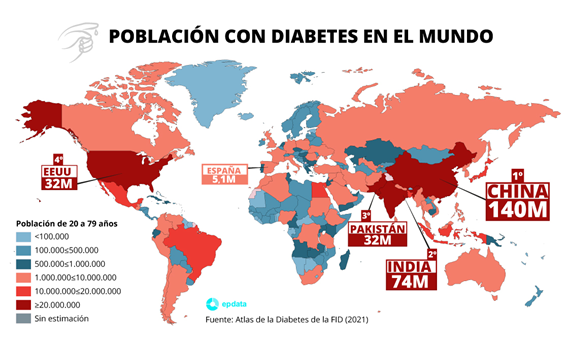
\includegraphics[width=0.8\textwidth]{img/imagen_poblaciondiabetica.png}
    \caption{Población con diabetes en el mundo en 2021 según la FID.}
    \label{fig:poblacion}
\end{figure}



La diabetes puede producirse por dos razones: o no hay suficiente insulina, o bien el cuerpo no responde de forma apropiada a ella. Bajo el primero de los casos, es el páncreas quien no produce la insulina de forma adecuada, por lo que es necesario la aportación de insulina externa para procesar y regular la glucosa en el cuerpo. Si este no responde a ella, lo que nos sitúa en el segundo caso, significa que el hígado no reconoce la insulina que está en el organismo y por tanto, continúa produciendo cantidades inadecuadas de glucosa. Este hecho se conoce como resistencia a la insulina.

\subsection{Tipos de diabetes}
Se describen a continuación los principales tipos de diabetes.

\textbf{Diabetes tipo 1 (DM1)}

Presenta un carácter autoinmune, donde el sistema inmunológico del organismo ataca y destruye las células beta del páncreas, lo que las impide producir insulina, ver Figura \ref{fig:tipos_diabetes}. Por tanto, los pacientes diabéticos de tipo 1 requieren de la administración de insulina externa a través de inyecciones o bombas de insulina. Es la más registrada en niños y adultos jóvenes. Es el caso de este estudio.

\textbf{Diabetes Tipo 2 (DM2)}

Se caracteriza por la resistencia a la insulina y una producción insuficiente de esta, siendo la forma más común de diabetes. Suele ir acompañada de obesidad. A diferencia del caso anterior, las células del cuerpo si que responden a la insulina, pero no lo hacen de forma eficaz, lo que desemboca en niveles elevados de glucosa en sangre (Figura \ref{fig:tipos_diabetes}). La enfermedad parece estar ampliamente relacionada, además de con el sobrepeso,  con otros factores del estilo de vida, como la falta de actividad física o una dieta poco saludable. Por tanto, los pacientes no suelen requerir de inyecciones de insulina, sino que el tratamiento engloba la dieta, el ejercicio y la medicación (donde destacan los antidiabéticos orales). 

\textbf{Diabetes gestacional}

Esta modalidad es un tipo especial de diabetes que se desarrolla durante el embarazo, y se caracteriza por presentar resistencia a la insulina, que parece estar causada por cambios hormonales. A pesar de que la diabetes gestacional suele desaparecer tras el parto, se ha relacionado con un mayor riesgo de que estas mujeres desarrollen diabetes tipo 2 en el futuro. Se puede obtener más información en  \cite{giarllarielli2023diabetes}.

\begin{figure}[h]
    \centering
    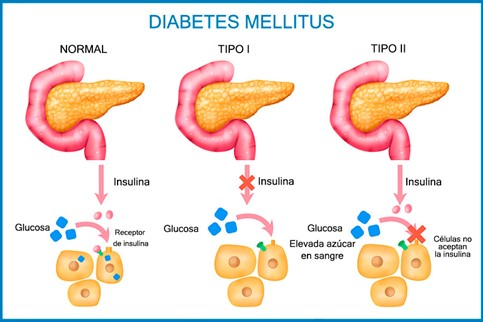
\includegraphics[width=0.6\textwidth]{img/imagen_tipos_diabetes.jpg}
    \caption{Interacción glucosa - insulina sin diabetes y con diabetes.}
    \label{fig:tipos_diabetes}
\end{figure}

\subsection{Rangos diabéticos}

Se incluyen a continuación los rangos que delimitan la diabetes \footnote{Obtenidos de \cite{mayoclinic_prediabetes}}: 

\begin{table}[htbp]
    \centering
    \caption{Valores estipulados para el paciente base.}
    \begin{tabular}{|c|c|c|}
        \hline
          & Ayunas & Tras ingesta  \\
        \hline
        Valores normales & 70-100 mg/dL & <180 mg/dL  \\
        Prediabetes & 100-125 mg/dL & 180-200 mg/dL \\
        Diabetes & >125 mg/dL & >200 mg/dL \\
        \hline
    \end{tabular}
    \label{tab:rangos_diabeticos}
\end{table}

\section{Pruebas glucémicas}

La medición de la glucosa sanguínea constituye el marco para el tratamiento eficaz de hiperglucemias e hipoglucemias en el organismo, así como para el seguimiento de pacientes con patologías relacionadas, incluso, con los avances tecnológicos actuales, para el monitoreo del ejercicio y otras perturbaciones \cite{gygliola2020glucose}. Su clasificación se basa en el método de administración empleado. Así, destacan dos pruebas, la de tolerancia oral a la glucosa y la de tolerancia intravenosa de la glucosa.
La prueba \textbf{Intravenous Glucose Tolerance Test (IGVTT)} es un test médico utilizado para evaluar cómo el cuerpo maneja la glucosa administrada por vía intravenosa. Se emplea principalmente para el diagnóstico de diabetes, aunque también sea útil para identificar otras condiciones relacionadas con la glucosa e insulina. Se administra una cantidad específica de glucosa al organismo mediante una vía, y posteriormente se toman muestras de sangre en intervalos regulares para medir los niveles de glucosa e insulina. Esta prueba permite una evaluación detallada de la función beta-pancreática y de la sensibilidad a la insulina, y, a diferencia de otras pruebas, es más controlada, ya que evita las variaciones en la absorción intestinal de la glucosa.\label{sec:IGVTT} 
La prueba de \textbf{tolerancia oral a la glucosa OGTT} emplea la vía oral para la administración de glucosa. Su principal uso es el diagnóstico de la diabetes tipo 2, pero se usa una variante de esta para identificar diabetes gestacional. Una vez pasado el intervalo de tiempo necesario, se procede de la misma forma que en la anterior prueba, es decir, mediante la extracción de sangre, lo que permite medir los niveles glucémicos. La OGTT identifica modalidades diabéticas clasificando la ingesta del paciente en función de su edad y condición (ver Figura \ref{fig:tipos_OGTT}).  Mientras que en adultos se estima una solución de unos 8 onzas con 75 gramos de azúcar, para niños, la dosis se calcula en función de su peso (1,75 g/kg), con una dosis máxima de 75 gramos. A diferencia de estas dos pruebas, cuya duración suele ser de 2 horas, existe una tercera modalidad empleada para las embarazadas, que utiliza una solución de 8 onzas con 100 gramos de azúcar, y dura 3 horas. \label{sec:OGTT}
\clearpage
\begin{figure}[htbp]
    \centering
    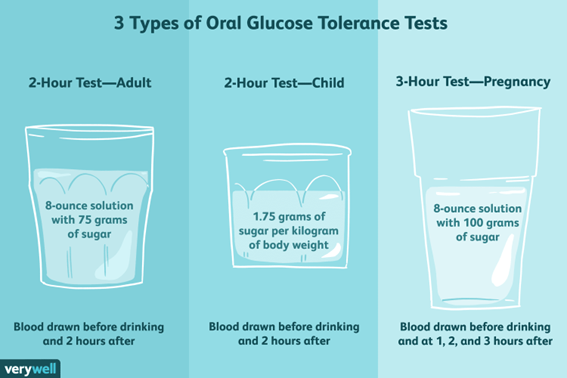
\includegraphics[width=0.75\textwidth]{img/tipos_OGTT.png}
    \caption{Tipos de pruebas de Tolerancia Oral a la Glucosa según el paciente implicado.}
    \label{fig:tipos_OGTT}
\end{figure}

\section{Monitorización y regulación de la glucosa}

\textbf{Sistemas de monitorización }

Se trata de dispositivos que obtienen una lectura de los valores glucémicos del paciente, mediante su monitorización. Se clasifican en tres:
\begin{enumerate}
    \item[-] Monitores de glucosa en sangre (BGM) son los más sencillos y requieren de una gota de sangre del paciente, obtenida mediante una punción del dedo. La sangre se aplica a una tira reactiva insertada en el medidor, que luego muestra la lectura de glucosa. 
    \item[-] Monitores continuos de glucosa (CGM) emplean un sensor insertado bajo la piel, generalmente bajo el brazo, que mide los niveles de glucosa en el líquido intersticial cada pocos minutos. Los datos obtenidos se envían a un dispositivo. A diferencia del monitor anterior, proporciona datos continuos, pero necesitan ser remplazados regularmente. \label{sec:CGM}
    \item[-] Monitores de glucosa flash (Flash Glucose Monitor), similares a los anteriores, a diferencia de que es el propio paciente quien debe escanear el sensor con un lector para poder obtener la lectura. 
\end{enumerate}

Se incluyen en la Figura \ref{fig:sist_mon_2022} los sistemas de monitorización de glucosa  (MCG) comercializados en España en 2022 según \cite{revistadiabetes_monitorizacion_glucosa}:

\begin{figure}[h]
    \centering
    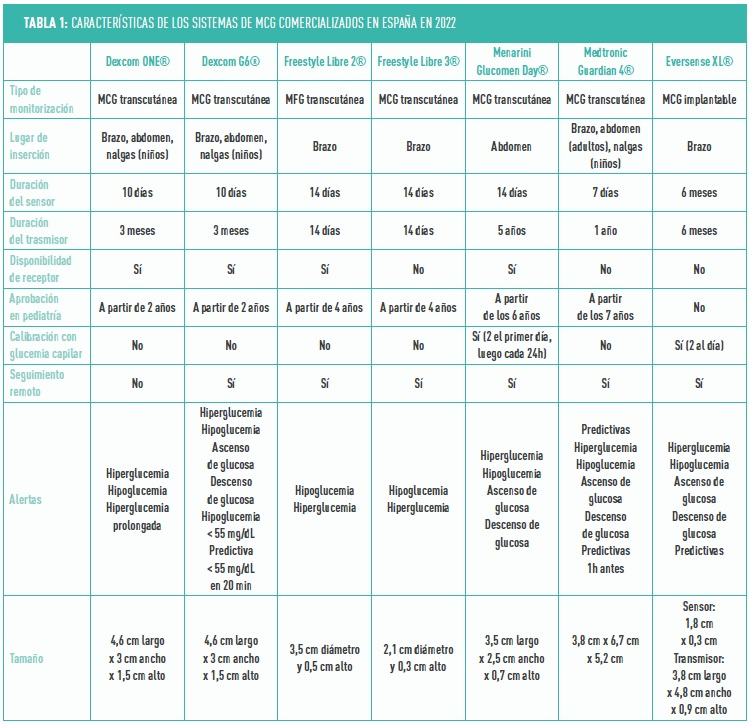
\includegraphics[width=1\textwidth]{img/comercializados.jpg}
    \caption{Sistemas de monitorización de glucosa comercializados en España en 2022.}
    \label{fig:sist_mon_2022}
\end{figure}

\textbf{Bombas de insulina} \label{sec:bomba}

Se trata de dispositivos que administran al organismo insulina, llamada insulina exógena, de manera continua o en dosis, a través de un catéter insertado debajo de la piel. El objetivo de este tratamiento es imitar el funcionamiento del páncreas de una persona sin diabetes. Funcionan de manera similar a un páncreas artificial, proporcionando una infusión constante de insulina basal (programada previamente por el equipo diabetológico, el paciente y/o su familia basándose en los controles de glucemia), así como dosis adicionales o "bolos" de insulina en momentos específicos, como en las comidas, según las necesidades del usuario. Estos bolos también se emplean para corregir las hiperglucemias \footnote{Información obtenida de \cite{FundacionParaLaSalud}.}.
Basándose en los datos de glucosa proporcionados por sistemas de monitorización, como el CGM mencionado anteriormente (Sección \ref{sec:CGM}), se pueden ajustar las configuraciones de esta bomba para adaptarse a necesidades individuales de cada paciente, programando mediante sistemas de control, por ejemplo, diferentes tasas de administración de insulina según la hora del día, la actividad física, etc. 
Entre las principales ventajas de las bombas de insulina, se encuentran cuatro:
\begin{enumerate}
    \item Permite ajustar mejor las diferentes necesidades de insulina que existen en el día gracias a la capacidad para programar las perfusiones basales.
    \item La bomba utiliza análogos de insulina de acción rápida, lo que asegura un efecto más predecible, en comparación con las insulinas de acción lenta o intermedia.
    \item Generalmente, se reduce el riesgo de hipoglucemias graves.
    \item Ha demostrado en diferentes estudios una mejoría en la calidad de vida del niño/adolescente y de su familia. Esta mejora se debe fundamentalmente a la flexibilidad horaria que ofrece.
\end{enumerate}

Sin embargo, también cuenta con algunas desventajas:
\begin{enumerate}
    \item Durante la terapia con bomba el depósito de insulina es muy escaso. Por este motivo se es más susceptible de presentar cetoacidosis en el caso de interrupción en el suministro de insulina.
    \item La bomba se debe llevar las 24 horas del día lo que para algunas personas supone una mayor “atadura” a su diabetes.
    \item Supone mayor gasto que la terapia con múltiples dosis de insulina.
\end{enumerate}


\textbf{Insulina exógena} 

Las insulinas se clasifican atendiendo, principalmente, a la duración de sus efectos así como a la rapidez de su acción, distinguiendo la acción rápida, corta, intermedia, larga o muy larga. Más comúnmente, esta clasificación se reduce a 3 tipos de insulina exógena: acción rápida, media y prolongada. \label{sec:ins_ex}

\begin{enumerate}
    \item[-] \textit{La insulina de acción rápida} produce efecto entre los 5 y 20 minutos desde la administración, ya que se absorbe rápidamente desde el tejido adiposo. Esta cifra resulta un tiempo muy reducido, mientras que su pico de acción se produce aproximadamente a la hora o dos horas del inicio. Su duración en el organismo es de unas 4-6 horas. Se emplea para regular los niveles de glucosa durante las comidas, o bien para corregir niveles altos de esta en sangre.
    Unas pocas unidades pueden durar 4 horas o menos, mientras que 25 o 30 unidades pueden durar 5 a 6 horas. Destacan la insulina lispro, la aspart y la glulisina; y su uso es cada vez más extendido. \label{sec:ins_rap}
    \item[-] \textit{La insulina de acción intermedia} muestra el inicio de acción más tarde, pues se absorbe más lentamente (entre la primera y la segunda hora), así como su pico de acción (a las 4-12 h). Sin embargo, su duración es sustancialmente mayor, alcanzando las 12-18 horas. Se usa para controlar el azúcar por la noche o bien entre las comidas. Destaca la insulina NPH.
    \item[-] \textit{La insulina de acción prolongada} se administra a pacientes diabéticos tipo 1 cuyo valor de insulina ha de mantenerse constante para todo el día. El inicio de la acción se produce tras 1 hora de la ingesta aproximadamente y, a diferencia del resto de insulinas, no experimenta picos de acción, sino que muestra un comportamiento estable. En general, se usa para controlar el azúcar a nivel diario. Ejemplos de esta insulina son Glargina y Detemir. \label{sec:ins_prol}
\end{enumerate}

\textbf{Páncreas artificial} 
\label{sec:pancreas_artificial}

Un páncreas artificial es un sistema en lazo cerrado automatizado para la administración de insulina en el organismo que imita la manera en que un páncreas sano controla la glucosa en la sangre.
Este sistema está formado por tres componentes (ver Figura \ref{fig:pancreas_art} \footnote{Obtenido de \cite{vibora2017pancreas}}):
\begin{enumerate}
    \item[-] Un monitor continuo de glucosa o CGM anteriormente expuesto en la Sección \ref{sec:CGM}, que  lleva un registro de la concentración de glucosa en la sangre cada pocos minutos mediante un pequeño sensor que se inserta debajo de la piel. El sensor envía la información de forma inalámbrica a un programa almacenado en un teléfono inteligente o en una bomba de infusión de insulina. Este dispositivo garantiza la continua monitorización de las concentraciones de glucosa.
    \item[-] Un programa informático, que calcula cuánta insulina se necesita y envía una señal a la bomba de infusión de insulina cuando debe administrarse. Así, el programa mejora el control de la glucosa en la sangre ajustando automáticamente la cantidad de insulina que administra para mantener las concentraciones de glucosa en la sangre dentro del rango. El modelado del comportamiento de la glucosa en el organismo mediante relaciones matemáticas, como las que se analizan en esta memoria, permiten diseñar sistemas de control adecuados y eficientes que será los que se implementen como parte del programa informático. Precisamente, el estudio de los modelos matemáticos y los sistemas de control más sencillos son el objetivo de este trabajo.
    \item[-]  La bomba de infusión de insulina, que administrará pequeñas dosis de insulina a lo largo del día cuando las concentraciones de glucosa en sangre no estén dentro de su rango objetivo (Sección \ref{sec:bomba}).
\end{enumerate}

\begin{figure}
    \centering
    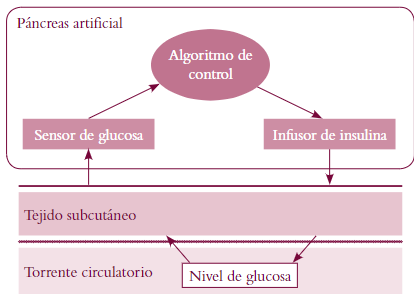
\includegraphics[width=0.65\linewidth]{img/pancre.PNG}
    \caption{Sistema de control del páncreas artificial.}
    \label{fig:pancreas_art}
\end{figure}

Existen diferentes tipos de sistemas de páncreas artificial, entre ellos: 
\begin{enumerate}
    \item[-] \textit{Sistemas de umbral de suspensión y de suspensión predictiva}, que pueden suspender de forma temporal la administración de insulina si la concentración de glucosa en sangre es muy baja, y evitar así una posible hipoglucemia.
    \item[-] \textit{Sistemas de insulina}, de carácter híbrido, que ajustan automáticamente las dosis de insulina en función de los valores leídos gracias al sistema de monitorización. Para estos sistemas, es necesario que el paciente cuente las concentraciones de ingesta y calcule la dosis necesaria para las comidas.
    \item[-] \textit{Sistemas hormonales duales}, en desarrollo, que emplean la insulina y el glucagón para reducir y aumentar las concentraciones de glucosa en sangre, respectivamente. Este comportamiento simula el del páncreas, y se estiman buenos resultados para ellos. 
\end{enumerate}

Mediante el empleo de modelos matemáticos que explican la interacción glucosa – insulina, se pretende en este análisis estudiar el comportamiento de la glucosa en el organismo, así como emplear estrategias de control para regular los niveles basales glucémicos.

\section{Modelos matemáticos del sistema glucorregulatorio}

\subsection{El Modelo de Ackerman}

\subsubsection{Contexto, funcionamiento y finalidad del modelo}

Constituye el primer intento de modelización de los procesos fisiológicos durante la metabolización de la glucosa, y se llevó a cabo en los años 60. Se trata de un modelo lineal cuya finalidad era la detección de la diabetes.
El Modelo de Ackerman se basa en la prueba OGTT de tolerancia oral a la glucosa (explicada en la Sección \ref{sec:OGTT}), cuyas mediciones servirán para obtener el diagnóstico de la enfermedad. El objetivo además era construir un modelo que describiese con precision el sistema regulador de la glucosa en la sangre durante la prueba OGTT. Además del empleo de esta prueba, se debe medir el péptido C para calcular la secreción de insulina, ya sea por desconvolución o modelado matemático.
Este modelo emplea la información proporcionada por dos concentraciones sanguíneas: la concentración de la glucosa y la de la insulina, englobando esta ultima un conjunto de hormonas. En \cite{ackerman1965model}, Ackerman interpretará que las hormonas que hacen disminuir la concentración de glucosa incrementarán la insulina, mientras que las que hacen el efecto contrario (elevar la glucosa), disminuirán los niveles de insulina. Por tanto, su conocimiento sobre la fisiología de la insulina y la glucosa en nuestro organismo fue clave para desarrollar el modelo. Aun así, como todos los modelos, presenta inconvenientes, principalmente en relación con el tiempo transcurrido respecto a la ingesta de glucosa.

\subsubsection{Ecuaciones y parámetros del Modelo de Ackerman}

El modelo es muy simple ya que requiere un número limitado de muestras de sangre durante la prueba OGTT. Da origen a un sistema de ecuaciones diferenciales prestando atención a dos concentraciones:

\begin{enumerate}
    \item[-] la concentración sanguínea de glucosa G(t), y
    \item[-] la concentración de insulina en plasma I(t).
\end{enumerate}

Las dos ecuaciones del modelo son:

\begin{equation}
\frac{dG(t)}{dt} = -p_1 (G(t)-Gb)-p_2 (I(t)-Ib)
\end{equation}

\begin{equation}
\frac{dI(t)}{dt} = p_4 (Gb-G(t))-p_3(I(t)-Ib) 
\end{equation}

En ellas, $p_1$, $p_2$, $p_3$ y $p_4$ son parámetros del modelo, mientras que $G_b$ e $I_b$ son los niveles de glucosa e insulina basal, respectivamente. 

	

\subsection{El Modelo Mínimo de Bergman}
\subsubsection{Contexto, funcionamiento y finalidad del modelo}
Este modelo aparece en 1980 de la mano de Richard N. Bergman y su equipo, y representa el verdadero inicio del modelado de las dinámicas glucosa - insulina. 
Su aparición se debe al aumento de los trastornos de sensibilidad de los tejidos a la insulina en diversas condiciones patológicas, como la diabetes (aunque también la obesidad o las enfermedades cardiovasculares), lo que hizo necesario trabajar en la cuantificación, mediante un proceso no invasivo, de la sensibilidad a la insulina. Se desarrolló entonces una prueba denominada con las siglas IVGTT (Sección \ref{sec:IGVTT}) para medir esta sensibilidad, basada en la administración intravenosa de un bolo de glucosa y el muestreo frecuente de las concentraciones tanto de glucosa como de insulina en el paciente. La interpretación de esta prueba se lleva a cabo mediante el modelo fisiológico que titula este apartado: el Modelo Mínimo.

Este modelo interpreta el organismo como un único compartimento, que posee una concentración basal tanto de glucosa como de insulina. Se basa en dos partes: 
\begin{enumerate}
    \item Estudia la cinética de la glucosa; es decir, describe la evolución (en tiempo) de la concentración plasmática de glucosa. Responde a la pregunta de cómo reacciona la concentración de glucosa a la acción de la insulina.
    \item Analiza la cinética de la insulina; lo que implica la medición de la concentración de insulina en el plasma en función del tiempo. Esto se traduce en la dinámica de liberación de insulina pancreática en respuesta al estimulo de un aporte de glucosa. Responde a la pregunta de cómo reacciona la insulina a la concentración de la glucosa en sangre. Introduce además el efecto de una nueva variable: la insulina activa, X(t).  De naturaleza “artificial”, se encuentra relacionada con dicha concentración insulínica pero que no coincide exactamente con ella.
\end{enumerate}

El análisis del comportamiento del sistema glucorregulatorio ha sido llevado a cabo mediante este modelo, y el procedimiento se encuentra en las siguientes secciones.

\section{La ingeniería de control}

La ingeniería de control se define por Jose García - Tirado en \cite{tirado2016ingenieria} como la disciplina que hace uso de la teoría de control para diseñar sistemas que garanticen el comportamiento deseado de otros. La \textit{teoría de control} estudia, por tanto, el comportamiento de estos sistemas dinámicos y la manera de lograr que se comporten como se desea. El término \textit{sistema} en este contexto se refiere a un mundo donde se producen tanto entradas (perturbaciones, exitaciones) como salidas (que se denominan respuestas).

\subsection{Principios básicos de la ingeniería de control}

La ingeniería de control se basa en ciertos principios básicos. 

La \textit{\textbf{estabilidad del sistema}}, en primer lugar, consiste en la capacidad del sistema para mantener el comportamiento deseado a lo largo del tiempo, en respuesta a perturbaciones o bien a cambios en las condiciones iniciales. Un sistema estable volverá a su estado de equilibrio tras la perturbación. En este contexto, un sistema con capacidad inherente de ajustarse y mantener su salida dentro de unos límites, sin necesidad de intervención externa se denomina \textbf{\textit{proceso autorregulador}}. Básicamente, un proceso autorregulado es aquel que tiende a estabilizarse pot si mismo. Es el caso del control de los niveles de la glucosa en el organismo.

La \textit{\textbf{retroalimentación}} es un mecanismo de control que permite a los sistemas ajustar su comportamiento. Mediante su uso, la información de entrada (\textit{variable de entrada}) se contrasta con un \textit{valor referencia} (llamado consigna de control) para darle una orden a la \textit{variable manipulada} y ejecutar así una acción correctiva. Se pueden dar dos tipos de retroalimentación:
\begin{enumerate}
    \item[-] Si la retroalimentación es \textit{negativa}, se reduce la diferencia entre la salida deseada y la salida real del sistema, estabilizando el sistema, y mejorando su precisión y resistencia a perturbaciones.
    \item[-] Si la retroalimentación es \textit{positiva}, al aumentar la diferencia entre la salida deseada y la real, se obtienen sistemas más inestables, generando respuestas oscilatorias, entre otras. 
\end{enumerate}

\subsection{Control de la glucosa en el organismo}

El el contexto biomédico, el conocimiento del funcionamiento de diferentes mecanismos fisiológicos del cuerpo humano en respuesta a perturbaciones ha experimentado una mejora significativa. Se entiende un \textit{ser vivo} como un conjunto de controladores automáticos internos que hacen su trabajo de manera colaborativa y distribuida, concepto comprensible, por ejemplo, con mecanismos básicos como la regulación del pH o de la temperatura, donde es el propio organismo quien regula estas variables y las mantiene en límites adecuados. Gracias al modelado matemático, se ha logrado una mejora en la comprensión de complejidad de los sistemas biológicos, destacando las metodologías automatizadas, que diseñan e implementan sistemas de control de manera automática, reduciendo la intervención manual y mejorando tanto la eficiencia como el desarrollo del sistema. Pese a que existen diferentes rutas para 'cerrar el lazo', J. Bondia estima en \cite{bondia2010pancreas} que la más adecuada es la que comprende la monitorización continua de glucosa subcutánea (s.c -s.c) visible en la Figura \ref{fig:ruta_sc}, destacando respecto a otras rutas como la intravenosa o la intraperitoneal.
\clearpage
\begin{figure}[htbp]
    \centering
    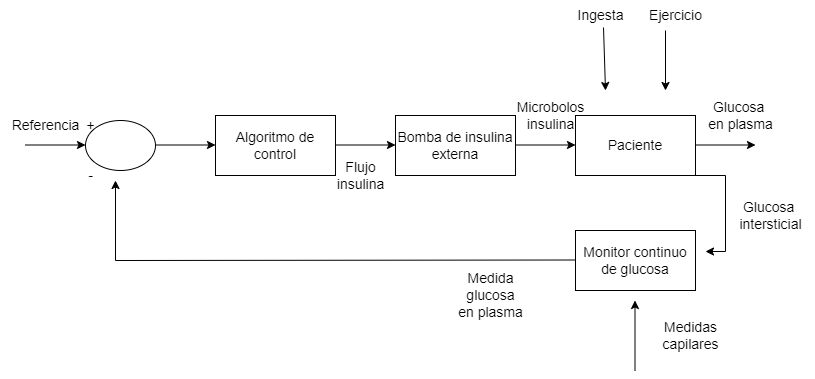
\includegraphics[width=1\linewidth]{img/ruta_sc.png}
    \caption{Lazo de control básico en la ruta s.c. -s.c. Fuente propia.}
    \label{fig:ruta_sc}
\end{figure}

J. Bondía también habla del problema de la sobreactuación, que es especialmente significativo en la compensación de ingestas, donde los errores son grandes. Es por ello, indica, que se emplea con frecuencia el anunciamiento de comidas, donde el paciente indica el instante y la cantidad de ingesta, como se hace en este trabajo. Pese a que, como se ha comentado, la ingesta no es una perturbación medible del todo, pues el flujo de absorción intestinal de glucosa solo se puede estimar en condiciones experimentales, la única información de la que se puede disponer es el instante de inicio de la ingesta y la estimación de la cantidad de hidratos de carbono por parte del paciente. Se muestra en la Figura \ref{fig:ruta_mod} el lazo de control modificado para esta condición, denominada, en la teoría de control, feedforward. Esta se combina siempre con una estrategia de realimentación como la vista antes (o feedback).
\clearpage
\begin{figure}[htbp]
    \centering
    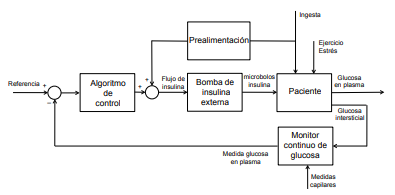
\includegraphics[width=1\linewidth]{img/ruta_mod.png}
    \caption{Lazo de control con anunciamiento de comida. Fuente propia.}
    \label{fig:ruta_mod}
\end{figure}

En el contexto de la glucosa, dispositivos como el páncreas artificial basan su funcionamiento en la ruptura del lazo de control natural. Este concepto se refiere a la estructura mediante la cual se regula el comportamiento de un sistema, mediante componentes que mantienen las variables dentro de rangos deseados. El estado natural de los sistemas de regulación del cuerpo humano es el lazo cerrado donde la acción de control se ajusta continuamente en función de la retroalimentación de la salida del sistema. La salida se mide y se compara con el valor deseado, y cualquier desviación (error) se utiliza para corregir la acción de control, mejorando la precisión y la estabilidad del sistema. Cuando se altera el comportamiento del organismo, como es el caso de la falta de insulina, que se traduce en hiperglucemia, se pasa al lazo de control abierto, donde la acción de control se aplica directamente sin usar retroalimentación para corregir el error entre la salida real y la deseada. Esto resulta en un estado de vulnerabilidad permanente hacia condiciones de alta o de baja concentración de glucosa.

Por tanto, la aplicación de principios de control automático en la diabetes representa un avance significativo y necesario en el área de la medicina, permitiendo un manejo más efectivo y preciso de la enfermedad, mejorando la calidad de vida de los pacientes y reduciendo el riesgo de complicaciones a largo plazo.

\clearpage
\section{Estado del arte y trabajos relacionados}

Respecto a las relaciones matemáticas de los mecanismos biológicos de la glucosa e insulina, la realidad es que actualmente existen multitud de modelos que simulan cada vez de forma más precisa su comportamiento. Además de los modelos clásicos, entre los que destacan los mencionados Modelos de Bergman y Ackerman, han surgido gran variedad de ellos.
\begin{enumerate}
    \item A nivel matemático, modelos basados en redes neuronales y Machine Learning, mediante la aplicación de nuevas inteligencias artificiales que son capaces de predecir los niveles de glucosa. Se incluyen entre ellos modelos basado en redes neruonales convolucionales CNN, que identifican patrones y mejoran las predicciones de los niveles de glucosa (\cite{carrillo2021long}), o 
    modelos de redes neuronales a corto plazo, como el 
    MLP (Multi Layer Perceptron), que es un tipo de red neuronal artificial que realiza predicciones a corto plazo de niveles de glucosa futuros permitiendo el mejor ajuste del tratamiento insulínico. Sus resultados son positivos, más información en \cite{allam2011recurrent}.
    \item En el ámbito probabilístico, modelos estocásticos que preveen las variaciones de la glucosa, entre los que se encuentran los modelos de Markov, procesos Gaussianos y modelos ARIMA. Se obtienen las probabilidades de que un paciente supere ciertos umbrales críticos en \cite{caperamodelo}, estimando relaciones relevantes entre los datos.
    \item En el ámbito médico, se han realizado grandes cohortes (estudios longitudinales), como el llevado a cabo por Leticia Marques da Silva Neto y otros \cite{da2024asociacion} en relación a la glucemia inestable y la mortalidad.
    \item En el ámbito farmacéutico, destacan las terapias combinadas de insulina con otros medicamentos \footnote{Más información en \cite{karam2024capitulo}}.
    \item A nivel tecnológico, se avanza en sistemas de monitoreo continuo de glucosa, así como, por excelencia, en el páncreas artificial. Destaca la empresa de tecnología médica Dexcom, cuyo mayor activo son los dispositivos Dexcom G6 y G7 de control de glucosa que permiten un monitoreo constante y a tiempo real. Su integración en aplicaciones móviles, así como la configuración de múltiples ventajas como alarmas y alertas personalizadas a los niveles glucémicos de cada paciente consolidan este producto como uno de los más potentes del mercado. Dexcom G7 se ha consolidado como el sistema MCG más rápido del mercado, pues requiere unicamente de 30 minutos para calentase, además de haber reducido un 60\% su tamaño respecto del anterior. Muy recientemente se ha aprobado la comercialización de un sistema Dexcom para diabéticos tipo 2 \cite{infobae_monitor_glucosa}, que es de venta libre, a diferencia del resto, que son bajo receta. Los sensores FreeStyle también permiten llevar un control continuo de los niveles de glucosa, y recientemente se ha estimado que los diabéticos tipo 2 con esta tecnología combinada con tratamientos con antagonistas del GLP 1 obtienen mejores resultados que solo con estos antagonistas (\cite{immedicohospitalario_freestyle}).
\end{enumerate}

Respecto al páncreas artificial, en el mes de abril se aprobó un nuevo páncreas para diabéticos tipo 1 que reduce los esfuerzos del paciente. Se trata de un sistema híbrido en lazo cerrado que adecua por si mismo los niveles de glucosa en el organismo, alejando al paciente de la preocupación ante esta posible situación. Este sistema emplea un sensor subcutáneo para monitorear los niveles de azúcar en sangre y una bomba de insulina inalámbrica para su administración \footnote{Para más información, consultar en \cite{gizmodo_pancreas_artificial}.}.
